\documentclass[11pt]{article}
\usepackage[a4paper,margin=22mm]{geometry}
\usepackage[T1]{fontenc}
\usepackage{lmodern}
\usepackage{graphicx,booktabs,array,amsmath,amssymb,url}
\usepackage[numbers,square,sort&compress]{natbib}
\usepackage[hidelinks]{hyperref}
\graphicspath{{figures/}}
\providecommand{\bibcommenthead}{}
\providecommand{\botrule}{\bottomrule}
\renewcommand{\footnotetext}[1]{\par\smallskip{\footnotesize #1}}
\renewcommand\thesection{S\arabic{section}}
\renewcommand\thefigure{S\arabic{figure}}
\renewcommand\thetable{S\arabic{table}}
\renewcommand\theequation{S\arabic{equation}}
\setlength{\parskip}{4pt}
\emergencystretch=3em
\begin{document}
\begin{center}{\Large Supplementary Data}\\[4pt]
Auditing cross-cohort feature-selection benchmarks: cohort composition and tissue-context-dependent confounding across kidney, liver and colon transcriptomes\\[4pt]
\textit{Briefings in Bioinformatics}\end{center}
Supplementary Notes S1--S10 carry the methods and results condensed out of the main text. Their wording is taken from the full-length version of the analysis, so section, figure and table numbers prefixed with S refer to this document, and others to the main text. Supplementary Files 1--7 are supplied separately.
\newcommand\suppnote[1]{\refstepcounter{section}\par\bigskip\noindent{\large\bfseries Supplementary Note \thesection. #1}\par\medskip}
\suppnote{Harmonisation, selection strategies and evaluation}\label{note:S1}
\subsection{Harmonisation}\label{sec:harmonisation}

Entrez Gene ID was used as the hub identifier because GSE104948 and GSE104954 use the Brainarray
ENTREZG custom CDF, so their probe identifiers already are Entrez IDs and the tightest cohort
suffers no mapping loss. Platform probes were mapped through GEO \texttt{.annot} files (GPL571,
GPL96, GPL8300, GPL6480), the GPL17586 platform table, and NCBI \texttt{gene\_info} for symbol-
and Ensembl-keyed matrices. Probes mapping to more than one gene were dropped. Where several
probes mapped to one gene the probe with the highest mean expression was retained (max-mean
collapse), a rule fixed before any analysis and applied identically everywhere, because changing
it invalidates every stability count computed on the resulting space.

The intersection over the four original discovery cohorts is 9,900 genes; adding the compartment
cohorts costs nothing since they share platforms. GSE294519 was mapped into this frozen space
rather than triggering re-derivation, and covers 98.5\% of it.

All cross-cohort operations use per-cohort gene-wise $z$-scores. Value scales differ
fundamentally between cohorts (GSE30528 and GSE30529 are mean-centred and negative; others are
positive log-scale), so raw values are never pooled. The $z$-scoring uses no label information,
so applying it to a held-out cohort is unsupervised domain alignment, not leakage.

\subsection{Selection methods}\label{sec:selectors}

Four strategies were compared, all on the same gene space and the same folds.

\textbf{DEG\_meta.} Per-cohort Welch $t$-statistic combined across cohorts by Stouffer's method
weighted by $\sqrt{n}$ \cite{whitlock2005}. The plain effect-size approach.

\textbf{WGCNA\_hub.} Soft-thresholded correlation network, module defined by gene--trait
correlation, genes ranked by intramodular connectivity: a connectivity-based hub ranking in the
manner of WGCNA \cite{langfelder2008}, of the kind used by prior DKD work \cite{feng2021}. It is
implemented directly rather than called from the reference package, and it departs from the
canonical pipeline in three respects: the soft power is fixed at $\beta = 6$ rather than chosen
by the scale-free topology criterion, modules are defined by gene--trait correlation rather than
by dynamic tree cut on the topological overlap matrix, and hubs are ranked by intramodular
connectivity rather than by module membership. We do not claim this reproduces WGCNA. Table~3 of the main text states element by element what is shared and what is not; Supplementary File~1 rebuilds the comparator across those axes and shows that the ranking behaviour Section~\ref{sec:modulesize} rests on is unchanged in every variant.



\textbf{RBS.} Cross-cohort stability selection (robust biomarker score), used here as an instrument rather than
proposed as a contribution: it stands in for the family of stability-selection approaches
\cite{meinshausen2010} so that the benchmark contains a representative of that family, and no
claim of novelty attaches to it. Bootstrap selection is run inside each cohort separately and
aggregated across cohorts, never on the pooled matrix. In the headline benchmark the inner selector is ReliefF, run on $B = 200$ class-stratified bootstrap replicates per cohort at $K = 50$. Let $\pi_{cj}$ be the fraction of those replicates of cohort $c$ in which gene $j$ is selected. The four components are importance $I_j$, the selector score of gene $j$ divided by the largest score in the same replicate, averaged over replicates and cohorts, so that a gene the selector never touches scores zero; stability $S_j = M^{-1} \sum_c \pi_{cj}$; cross-cohort reproducibility $R_j$; and perturbation robustness $P_j$, the selection frequency of gene $j$ over 40 refits per cohort under class-stratified 70\% subsampling, Gaussian noise at half the gene-wise standard deviation, masking of 20\% of genes, and a synthetic batch shift, computed only for the 300 genes ranked highest by $I_j S_j R_j$ so that perturbation stress-tests candidates rather than discovers them:

\begin{equation}
R_j = \delta_j \exp\Bigl( \frac{1}{M} \sum_{c} \log (\pi_{cj} + \epsilon) \Bigr) , \qquad
\mathrm{RBS}_j = \delta_j \exp\Bigl( \frac{\sum_k w_k \log (V_{kj} + \epsilon)}{\sum_k w_k} \Bigr) ,
\label{eq:rbs}
\end{equation}

where $V_{\cdot j} = (I_j, S_j, R_j, P_j)$, $w = (1, 1, 2, 1)$, $\epsilon = 10^{-3}$ inside $R_j$ and $10^{-6}$ in the combination, and $\delta_j \in \{0, 1\}$ is the
sign-concordance gate, equal to $1$ only when $g_{cj}$ carries the same non-zero sign in every
cohort. The geometric mean requires a gene to be adequate on all four components rather
than to buy its way in on one, and the gate is hard rather than a soft penalty. Baseline selectors within the bootstrap were compared (univariate
$F$, LASSO \cite{tibshirani1996}, elastic net \cite{zou2005}, mRMR \cite{peng2005}, ReliefF \cite{kononenko1994}, random forest \cite{breiman2001}, Boruta \cite{kursa2010}), all implemented directly rather
than through packages that pin older \texttt{numpy}/\texttt{scikit-learn} versions.

\textbf{RBS\_orth.} RBS after residualising every gene on a per-sample handling score
(the main-text section \textit{Confounder score, corrections and control definition}).

Two cohort sets are used and the distinction matters when reading the tables below. The headline
benchmark and its nulls run on the four cohorts fixed before the analysis began (GSE30528,
GSE96804, GSE104948, GSE142025). The cohort-composition sweep of the main-text section \textit{Reproducibility verdicts depend on cohort composition}
adds GSE294519 as a fifth, because that analysis exists precisely to vary the cohort set and
a wider set of compositions makes it stronger.

Evaluation is leave-one-dataset-out (LODO). Write the harmonised cohorts as $D_1,\dots,D_M$. For held-out cohort $m$ the training set is $T_m = \bigcup_{j \neq m} D_j$; a selection strategy $S$ returns the top-$K$ gene set $G_m^{(K)} = S(T_m,K)$; a plain $L_2$ logistic model $f_m$ is fitted on $T_m$ restricted to those genes and assigns each sample $i \in D_m$ a score $s_i = f_m(x_i)$. The classifier is deliberately simple because the object of study is the features, not the classifier.

Let $P_m$ and $N_m$ be the case and control samples of $D_m$, with $n_1 = |P_m|$ and $n_0 = |N_m|$. External AUROC is the Mann--Whitney statistic, ties counted as half:
\begin{equation}
\mathrm{AUROC}_m = \frac{1}{n_1 n_0}
\sum_{i \in P_m} \sum_{j \in N_m}
\Bigl[ \mathbf{1}(s_i > s_j) + \tfrac{1}{2}\mathbf{1}(s_i = s_j) \Bigr] ,
\label{eq:auroc}
\end{equation}
and the reported value is the mean over folds, $\overline{\mathrm{AUROC}} = M^{-1}\sum_{m=1}^{M} \mathrm{AUROC}_m$. The tie term matters here because several cohorts are small enough for scores to tie exactly.

The second axis is reproducibility, the agreement between the gene sets selected on different training sets:
\begin{equation}
J = \binom{M}{2}^{-1} \sum_{m < m'}
\frac{|G_m^{(K)} \cap G_{m'}^{(K)}|}{|G_m^{(K)} \cup G_{m'}^{(K)}|} .
\label{eq:jaccard}
\end{equation}
The two axes are reported separately throughout and are not interchangeable: the main-text section \textit{Reproducibility verdicts depend on cohort composition} shows they disagree.

\textbf{Effect size.} Every effect size reported here is Hedges' $g$ \cite{hedges1981}, the standardised
mean difference with the small-sample correction. For gene $j$ with case and control
groups of size $n_1$ and $n_0$,

\begin{equation}
g_j = \frac{\bar{x}_{1j} - \bar{x}_{0j}}{s_{p,j}} \Bigl( 1 - \frac{3}{4(n_1 + n_0) - 9} \Bigr) , \qquad
s_{p,j}^{2} = \frac{(n_1 - 1) s_{1j}^{2} + (n_0 - 1) s_{0j}^{2}}{n_1 + n_0 - 2} .
\label{eq:hedges}
\end{equation}

The specificity gate keeps genes with $|g_j| \ge 0.5$ in the diabetic-versus-other-
kidney-disease contrast, averaged over the two ERCB compartments.


\suppnote{Null controls, uncertainty and the random-signature null}\label{note:S2}
\subsection{Null controls and uncertainty}\label{sec:nulls}

Two nulls are computed per fold and per signature size. For the random-signature null, $B = 300$ gene sets $R_1,\dots,R_B$ of the same size $K$ are drawn uniformly from the same frozen gene space, and the model is refitted and rescored on the same fold with real labels. An observed AUROC is reported as its position in that null,
\begin{equation}
\pi_m = \frac{1}{B} \sum_{b=1}^{B}
\mathbf{1}\bigl( \mathrm{AUROC}_m^{(R_b)} < \mathrm{AUROC}_m \bigr) ,
\label{eq:percentile}
\end{equation}
never as the raw value. The second null permutes the case/control labels within each cohort and leaves everything else unchanged, so it measures what the evaluation returns when no signal exists at all. This control follows Venet et al.\ \cite{venet2011}, who showed that most random signatures are significantly associated with outcome in breast cancer.

All method comparisons use a paired patient-level bootstrap of $R = 40$ replicates, stratified by cohort and class, with the entire LODO evaluation, selection included, re-run inside each replicate. The interval is formed on the paired difference computed within a replicate,
\begin{equation}
\Delta^{(r)} = \overline{\mathrm{AUROC}}_{A}^{(r)}
- \overline{\mathrm{AUROC}}_{B}^{(r)} ,
\qquad r = 1,\dots,R ,
\label{eq:paired}
\end{equation}
and quoted as the 2.5th and 97.5th percentiles of $\Delta^{(1)},\dots,\Delta^{(R)}$. Pairing within the replicate is what makes the interval informative: the two methods see identical patients, so the cohort-to-cohort variance that dominates the marginal AUROC cancels. Resampling folds (3--5 units) or the pairwise
Jaccard values (which are correlated) does not support an interval. $R$ is small for a percentile interval because each replicate repeats the whole evaluation, selection included; it is set by compute, and the intervals should be read as bootstrap ranges whose finest resolvable two-sided $p$ is $2/R = 0.05$.

Cohort-composition sensitivity is assessed exhaustively: every subset of the five discovery
cohorts of size 2--5 (26 subsets) receives a complete benchmark, with 30 inner bootstrap replicates per cohort rather than the 200 of the headline run, since the sweep asks which method wins rather than for its score to the third decimal.


\subsection{Absolute AUROC is uninformative in this disease}\label{sec:auroc-null}

Randomly drawn 50-gene sets achieve external AUROC of 0.68--0.88 depending on the held-out
cohort, while permuting training labels gives approximately 0.50 (Table~\ref{tab:null},
Fig.~\ref{fig:null}). The signal is real, but which genes carry it is nearly immaterial. The DKD
programme is broadly co-expressed: among the 50 genes with the largest mean $|g|$ the mean pairwise
$|r|$ within a cohort is 0.51, against 0.25 for random gene sets of the same size, so most random
signatures inherit it. On the GSE142025 fold, random sets reach AUROC 1.000 at $K = 100$, making
that fold unable to discriminate methods at all.

\begin{figure}[htbp]
\centering
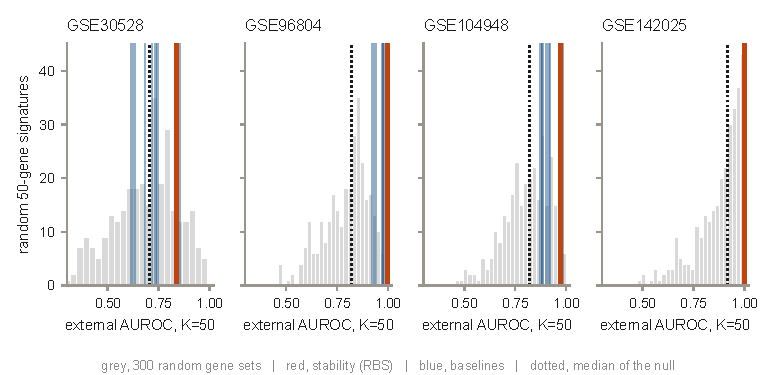
\includegraphics[width=\textwidth]{FigS1}
\caption{\textbf{Absolute AUROC is uninformative in this disease.} External AUROC for random
50-gene signatures, for permuted-label controls, and for the selected signatures, by held-out
cohort. Random signatures reach 0.68--0.88 depending on the fold; permuted labels sit at
approximately 0.50. A reported AUROC must be read against the random-signature band for its fold,
not against 0.5.}\label{fig:null}
\end{figure}


\begin{table}[h]
\caption{Random-signature and permuted-label nulls, by held-out cohort ($K = 50$)}\label{tab:null}
\begin{tabular}{@{}lll@{}}
\toprule
Held out & Random 50-gene AUROC & Permuted labels \\
\midrule
GSE30528  & 0.682 [0.385--0.923] & 0.52 \\
GSE96804  & 0.796 [0.597--0.946] & 0.47 \\
GSE104948 & 0.809 [0.602--0.962] & 0.55 \\
GSE142025 & 0.878 [0.654--1.000] & 0.49 \\
\botrule
\end{tabular}
\footnotetext{Brackets give the 5th--95th percentile over 300 random draws.}
\end{table}

A comparable random-signature phenomenon appears in a metabolomic layer, measured in
different patients by a different principle. In plasma from ST003255 (64 diabetic
nephropathy, 66 IgA nephropathy, 66 membranous nephropathy, 24 hypertensive nephropathy,
66 healthy), randomly drawn 20-metabolite sets reach a cross-validated AUROC of 0.913
against healthy controls, while a set selected inside each fold reaches 0.995 and permuted
labels give 0.50. Imputation, log transformation and scaling are fitted on the training
fold only and applied to the held-out fold, so no test sample contributes to the transform.
The signature size was fixed at 20 in advance; at 10 the selected set still clears the 95th
percentile of the null and at 50 it no longer does, which is itself the point: the margin
over the null, not the absolute figure, is what a comparison can rest on. This is a single
cohort evaluated by cross-validation rather than an independent replication, and we read it
as a cross-modal illustration that the reporting problem is not confined to transcriptomes.

Every AUROC reported below is therefore accompanied by its position in this null.


\suppnote{Procurement evidence: per-dataset values, single-nucleus control and heart}\label{note:S3}
\textbf{A note on what is and is not measured.} No DKD cohort we examined reports warm or cold
ischaemia time, fixation, or time to stabilisation. Procurement route is read from the sample
source annotation (needle biopsy versus nephrectomy or donor tissue), so the attribution to
pre-analytical handling is an inference, not a measurement. It rests on three things: the
association between procurement route and module level holds across nine datasets and four
platforms; the module does not separate two groups that share a procurement route, even when one
is diabetic and the other is not; and warm ischaemia is independently documented to induce
exactly these transcripts within minutes, including in kidney \cite{ma2012}, and ischaemia time is a documented driver of transcriptome variation across human tissues at scale \cite{ferreira2018}. Since this analysis was completed, an independent single-cell comparison of reference tissue sources within KPMP has reported the same dependence: stress-response genes are higher in nephrectomy and living-donor tissue than in percutaneous biopsies from healthy volunteers, and the choice of reference changes which genes are called differentially expressed \cite{menon2026}. We use
``procurement-associated'' throughout and reserve ``artifact'' for the interpretation, which the
data support but do not prove.

Across nine kidney datasets the IEG module tracks how tissue was obtained, not disease
(Table~\ref{tab:procurement}, Figure~2 of the main text). The Spearman correlation between
procurement (biopsy versus non-biopsy) and module level across all groups is $\rho = -0.752$,
$p < 0.001$.




\begin{table}[h]
\caption{Immediate-early module level by procurement route, across nine kidney
datasets}\label{tab:procurement}
\begin{tabular}{@{}llll@{}}
\toprule
Dataset & Biopsy & Non-biopsy & Difference \\
\midrule
GSE142025  & $-0.63$ & $+1.26$ & $-1.90$ \\
GSE104954  & $-0.23$ & $+1.37$ & $-1.60$ \\
GSE175759  & $-0.21$ & $+1.10$ & $-1.31$ \\
GSE96804   & $-0.39$ & $+0.80$ & $-1.19$ \\
GSE104948  & $-0.15$ & $+0.88$ & $-1.03$ \\
KPMP snRNA & $-0.33$ & $+0.64$ & $-0.97$ \\
GSE30529   & $-0.26$ & $+0.22$ & $-0.48$ \\
GSE30528   & $-0.19$ & $+0.13$ & $-0.32$ \\
GSE162830  & $+0.13$ & $+0.18$ & $-0.05$ \\
\botrule
\end{tabular}
\footnotetext{Values are the module mean $z$-score computed within each dataset.}
\end{table}

The KPMP single-nucleus data provide the decisive control because they contain both contrasts
with donor-level replication (27 DKD-proxy donors as defined in the main-text section \textit{Cohort assembly and audit}, 10 non-diabetic CKD, 12 reference, 6 nephrectomy donors;
statistics on donor $\times$ cell-type pseudobulk, Fig.~\ref{fig:singlecell}; the three
contrasts are tabulated in Supplementary File~4).

\begin{figure}[htbp]
\centering
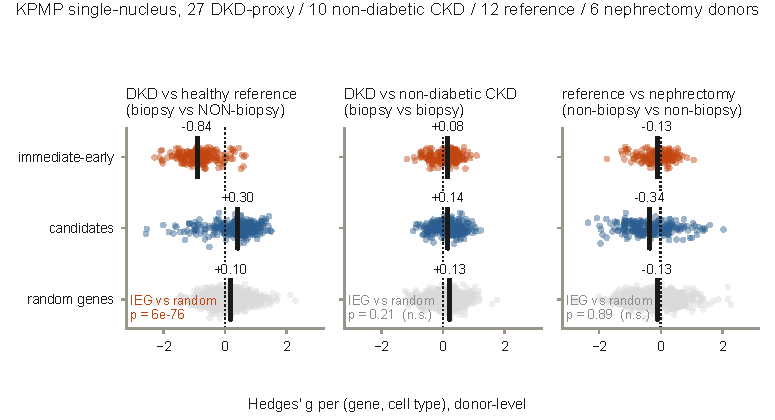
\includegraphics[width=\textwidth]{FigS2}
\caption{\textbf{A biopsy-versus-biopsy contrast removes the effect.} KPMP single-nucleus data
reduced to donor-level pseudobulk. Comparing DKD with non-diabetic CKD, both procured by needle
biopsy, gives $p = 0.21$; comparing DKD with non-biopsy reference tissue in the same resource
gives $p = 6.0\times10^{-76}$. The contrast is the negative control for
Figure~2 of the main text: when procurement is held constant the signal disappears, and it is
not a property of DKD.}\label{fig:singlecell}
\end{figure}


GSE162830, the single dataset where all 32 samples were processed identically (OCT,
$-80\,^{\circ}$C, laser microdissection), shows no procurement effect at all ($-0.05$), which is
what the interpretation predicts.

Because cases are biopsies and controls surgical tissue in every discovery contrast, this
confounder is shared across cohorts and therefore maximally reproducible. A criterion that
rewards cross-cohort consistency will rank it first: uncorrected RBS places 10 immediate-early
genes in its top 50.

This is organ- and protocol-specific, not universal, and the main text summarises it because it bounds the claim. In heart failure (GSE5406, 194
explanted ventricles versus 16 donor hearts) the module separates explant from donor only weakly
($g = -0.23$) and instead separates ischaemic from idiopathic cardiomyopathy, both explants
($p = 4\times10^{-8}$). Explanted and donor hearts undergo similar cardioplegia and cold storage,
whereas needle biopsies and nephrectomies differ substantially in warm ischaemia. The confounder
is a property of the procurement contrast, not of the gene module.


\suppnote{Why the connectivity criterion escaped the confounder}\label{note:S4}
The simulation uses a generative model with a disease block and a confounder block, each
with within-block correlation, cohort-specific effect heterogeneity ($\sigma_d$, $\sigma_c$ drawn once per cohort),
and a confounder correlated with case status by $\rho$. Block sizes, $\rho$, heterogeneity and
cohort count are swept. The stability arm was run both with a simplified stand-in and with the
actual RBS implementation; conclusions were identical.


\subsection{Why one method escaped the confounder, and why that is not
robustness}\label{sec:modulesize}

This section exists to close a loophole in Supplementary Note~S3 rather than to open a
second topic. If a widely used criterion simply avoids the confounder, the problem is less
serious than we claim. It does avoid it here, but for a reason that does not generalise.

The connectivity comparator placed no immediate-early genes in its top 50 while stability
selection placed 10. This exclusion alone does not establish robustness. In the real data 12 of 19 immediate-early genes are inside the disease-correlated
module and have high gene--trait correlation (\textit{DUSP1} $|gs| = 0.710$, among the highest in
the module), yet rank 790th of 990 by connectivity, because intramodular connectivity is a
\emph{sum} of adjacencies and therefore rewards membership of the largest coherent block: the
median block size (module genes with $|r| > 0.5$) is 19 for the immediate-early genes against 705
for the top 50 by connectivity, and 395 for the whole module.

This is not an artifact of how the comparator was implemented. Rebuilding it across every
combination of module definition (gene--trait correlation or clustering on the topological
overlap matrix), hub criterion (intramodular connectivity or module membership), adjacency
(signed or unsigned) and soft power ($\beta \in \{4, 6, 8, 12\}$, spanning both our value and
the $\beta \ge 10$ the scale-free criterion would select on these data) gives 32 variants, and
\emph{all 32 place no immediate-early gene in the top 50}. The WGCNA package itself, run with its
tutorial defaults on every fold of the cohort sweep, does not: in 9 of 75 folds (3 of the 30 distinct training combinations the folds evaluate) it
placed immediate-early genes in its top 50, up to 18 of 50, always where dynamic tree cut had
produced a small trait module (61 to 199 genes against a median of 588). Because the package ranks
by $|$kME$|$ within the chosen module, this is consistent with module-dependent exclusion rather
than a direct test of the summed-connectivity account; the median rank of an immediate-early
gene within its module ranges from 664 to 3{,}531. Under a signed network the immediate-early
genes are not module members at all, so the confounder is missed earlier still. Raising $\beta$
improves their rank without approaching the top 50, so our lower $\beta$ is conservative against
our own argument. Supplementary File~1 reports the full grid.

Simulation confirms the mechanism and shows that it reverses (Fig.~\ref{fig:blocksize}; the
paired differences are tabulated in Supplementary File~1).

\begin{figure}[htbp]
\centering
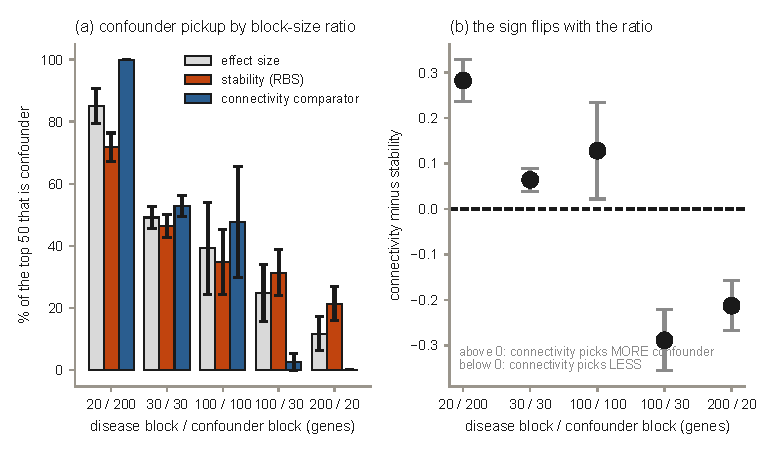
\includegraphics[width=\textwidth]{FigS3}
\caption{\textbf{Connectivity criteria are biased by module size, which is why one method
escaped.} Simulation sweeping the ratio between the size of the disease block and that of the
confounder block. \textbf{a} Percentage of the top 50 features that come from the confounder
block. \textbf{b} The difference between a connectivity criterion and a stability criterion,
which changes sign as the ratio crosses one. In the real data the immediate-early block contains
19 genes against 705 in the top-connectivity block, placing it in the regime where connectivity
misses the confounder for reasons unrelated to robustness. All seven configurations are
significant by Wilcoxon signed-rank on paired replicates.}\label{fig:blocksize}
\end{figure}


The sign tracks the block-size ratio; effect-size and stability criteria show no such dependence
(differences $-0.025$ to $+0.022$ across the same configurations). The connectivity comparator avoided the kidney
confounder because that confounder happened to form a small block. Where a confounder forms a
large programme, connectivity is the worst of the three.


\suppnote{Correction benchmark details and the seven inner selectors}\label{note:S5}
\subsection{Which corrections work}\label{sec:whichcorrections}

Corrections are compared on three axes at once: how much of the confounder survives, whether the
surviving signal is DKD-specific, and what the correction costs in external AUROC
(Table~6 of the main text, Figure~3 of the main text).






ComBat returns the same values as no correction in this implementation and evaluation setting.
Cohort-level batch adjustment alone cannot disentangle procurement from disease when the two are
confounded \emph{within} cohorts. RUVg with
empirically chosen controls also fails; the control set, not the framework, does the work.
Residualisation and surrogate-variable adjustment both succeed. Table~6 of the main text
reports identical fold-mean AUROCs to three decimal places for no correction and for
residualisation. In a separate patient-stratified paired bootstrap analysis with 200 replicates,
which resamples patients within each cohort and class and re-runs the whole leave-one-dataset-out
evaluation in every replicate at a reduced inner bootstrap ($B = 30$ rather than the 150 of the
fold means), the mean uncorrected minus residualised difference was $+0.079$ (95\% percentile
interval $-0.048$ to $+0.229$). This exploratory uncertainty estimate does not establish
performance preservation: a substantial loss remains compatible with the interval, whose tails are
imprecisely estimated.

The evaluation is not circular: the procurement flag derives from ERCB effect sizes, not from
module membership, and correlation with the handling score separates flagged from unflagged genes
at AUC $= 0.480$ (0.5 indicates independence).

The correction is not specific to the selector it was benchmarked with. Repeating the comparison with each of the seven inner selectors of Section~\ref{sec:selectors}, at $B = 40$ rather than 150 because the question is the direction of the change rather than its third decimal, the procurement-flagged fraction of the top 50 falls for every one of them (Table~7 of the main text), from 17.0--35.5\% to 3.5--12.5\%. The cost is not uniform. External AUROC rises for ReliefF (+0.021), falls by less than 0.05 for Boruta and mRMR, and falls by 0.05 to 0.11 for Elastic net, LASSO, Random forest and Univariate $F$. The removal is therefore a property of the correction, its cost a property of the selector, and a study adopting the correction should report that cost for the selector it uses.




\suppnote{Control-definition analysis by diagnosis and external checks}\label{note:S6}
\subsection{The control-group problem is not specific to diabetic kidney
disease}\label{sec:external}

Everything above concerns one disease, which leaves open whether the effect is a property of
diabetic kidney disease or of the design that every public kidney biopsy study shares. The ERCB
compartments answer this inside a single resource, because they contain eight biopsy diagnoses
alongside the same non-biopsy controls. We call the comparison that follows a \emph{control-
definition sensitivity analysis}: holding the case set fixed, it asks how far the ranking and
the effect-size conclusions move when the control group is replaced by an alternative that is
clinically defensible. It does not separate clinical from pre-analytical causes, and we do not
claim it does; procurement is our reading of why the two definitions differ here, supported
by the evidence in Supplementary Note~S3 rather than established by this comparison. For each diagnosis we formed the two contrasts the
argument turns on, namely diagnosis versus non-biopsy control and diagnosis versus the
remaining biopsy diagnoses, and counted genes reaching $|g| \ge 0.5$ (Table~8 of the main text). Seven of the
eight are reported; thin membrane disease was left out because its 9 cases give neither
contrast usable power.



Shrinking is not the whole of it. A signal that fell uniformly would leave the ranking, and
therefore the candidate list, unchanged; what happens instead is that the top of the ranking is
rebuilt (Figure~4 of the main text). Taking the 50 largest effects under each contrast, the two
lists share 1 gene in diabetic nephropathy and between 0 and 18 across the seven
diagnoses. The comparison holds the case set fixed and varies the control group; it is not
a within-patient pairing, for which no public data exist. Rank correlation over all 9,900 genes is 0.69 for diabetic
nephropathy, so the bulk of the transcriptome moves together while the extreme that feeds
selection does not. The movement has direction: myeloid and inflammatory genes fall (\textit{TYROBP}
31 to 678, \textit{CASP1} 16 to 603) while matrix genes rise (\textit{FMOD} 1264 to 4,
\textit{OLFML3} 5530 to 377). \textit{MOXD1} moves from 204 to 40; that is a change in
priority under a contrast with less procurement asymmetry, not evidence that it is a marker.




The consequence for a candidate list is direct. Running the same pipeline with and without
the handling-score correction returns 30 candidates each, sharing only 14
(Supplementary File~3). Which genes a study nominates is therefore set by how its control
tissue was obtained as much as by the disease.

Every diagnosis loses most of its signal, and diabetic nephropathy is unremarkable among them:
it ranks fourth of seven, and the median across the other six is 36\% against its 37\%. In IgA
nephropathy the 3,800 genes reaching $|g| \ge 0.5$ against non-biopsy controls fall to none.
The problem therefore belongs to the design rather than to the disease, and the argument of
Supplementary Note~S3 and~\ref{sec:whichcorrections} applies to kidney biopsy studies
generally. One qualification carries over from Supplementary Note~S3: the matched
comparator here pools the remaining diagnoses, and pooling can itself produce a result, so these
figures should be read as the pooled-comparator case.

Three datasets never used elsewhere in this work provide external checks of the candidate list.
In GSE20602, which compares nephrosclerosis glomeruli against tumour nephrectomy, the same
control type as GSE30528, the candidates move further in the diabetic contrast than in the
nephrosclerosis one (median $|g_{\text{DKD}}| - |g_{\text{NSC}}|$ of $+1.02$ against $-0.17$ for
the remaining genes, Mann--Whitney $p = 5.1 \times 10^{-18}$), which replicates the specificity
gate outside ERCB. In GSE111154 the candidates are already altered in early diabetic nephropathy
(permutation $p = 0.0015$), though with four patients per group this is weak. In GSE142153, blood
from diabetic nephropathy patients, the candidates are indistinguishable from random genes
($p = 0.80$): the signature is tissue-restricted, which supports its specificity and limits its
clinical accessibility at the same time.

The comparator behaves the same way in that metabolomic layer, which is the clearest
evidence that the recommendation is not specific to transcriptomics. Replacing the healthy
controls of ST003255 with the non-diabetic kidney disease patients of the same study drops the
random-set AUROC from 0.913 to 0.724, and the selected set clears its null by a wider
margin: 0.854 against a 95th percentile of 0.800, where against healthy controls it was
0.995 against 0.977. The reason is visible in the effect sizes. Across the 187 named metabolites the
diabetic-versus-healthy and other-kidney-disease-versus-healthy effect vectors correlate at
$r = 0.851$, so most of what separates these patients from healthy people is shared with kidney
disease in general. Twenty-nine metabolites survive the matched contrast at $q < 0.05$. A
disease-relevant comparator distinguishes diabetic-kidney-disease-associated changes from
metabolic changes shared across kidney diseases; it does not establish the procurement
mechanism seen in the transcriptome cohorts, which is a property of how those tissues
were obtained and has no counterpart in plasma.


\suppnote{Candidates and protein-level corroboration}\label{note:S7}
\subsection{What the pipeline returned, and what happened to it}\label{sec:candidates}

Applied without correction, the pipeline produced 30 specificity-gated candidates, of which two
(\textit{OLFML3}, \textit{PRSS23}) had no DKD literature. Three independent tests removed them:
the direction reversed in GSE175759, they were indistinguishable from random genes in the KPMP
confounder-matched contrast, and the corrected selector did not rank them. The corrected selector
instead recovered established DKD genes at a higher rate (20 of 30 already proposed as DKD markers
versus 13 of 30 uncorrected), including \textit{FMOD}, \textit{LUM}, \textit{MMP2} and
\textit{THBS2}; \textit{FMOD} and \textit{LUM} had previously been reported as
DKD hub genes \cite{feng2021}. A germline test against a Korean DKD genome-wide association study
(2,532 cases) with SNP-count-matched permutation nulls was a clean null (1 of 30 at empirical
$p < 0.05$, expected 1.5; Kolmogorov--Smirnov $p = 0.74$).

Figure~\ref{fig:candidates} shows what stands behind each of the 30, and why none
of them clears the bar. Two axes decide a biomarker claim: the gene must be strong in the data
and it must not already be in the DKD literature. Six candidates are strong but reported, six are
unreported but weak, and the cell requiring both is empty.

\begin{figure}[htbp]
\centering
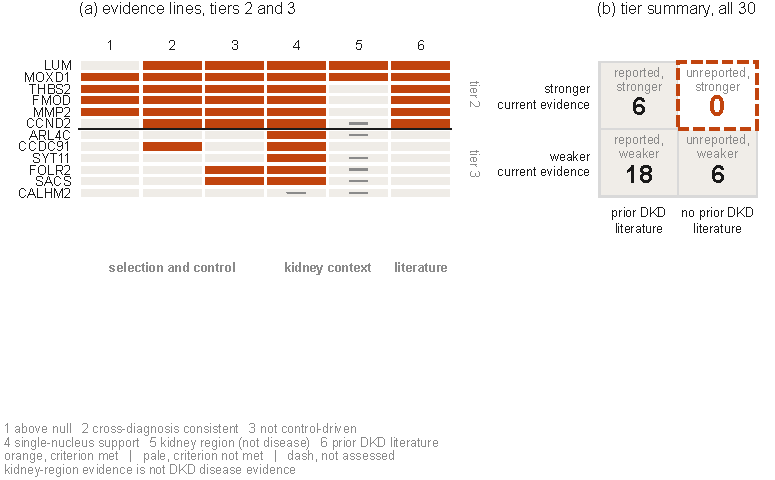
\includegraphics[width=\textwidth]{FigS4}
\caption{\textbf{Candidate evidence ledger.} \textbf{a} The 12 tier-2 and tier-3 candidates, which have either stronger current evidence or no prior DKD literature. The columns separate selection and control tests, human-kidney context, and literature status. Orange indicates a criterion met, pale a criterion not met, and a dash an assessment unavailable for that candidate; missing single-nucleus or regional-protein measurements are not scored as failures. The regional-protein column is the KPMP glomerulus-versus-tubulointerstitium contrast, which locates a protein rather than relating it to disease; it is not the diabetic-versus-non-diabetic protein evidence of Section~\ref{sec:proteome}, reported separately. The 18 tier-4 candidates are omitted here for legibility; Supplementary File~5 extends the matrix to all 30. \textbf{b} All 30 candidates classified by current evidence strength and prior DKD literature. The stronger-evidence/no-prior-literature cell is empty under the criteria fixed before the evidence was read.}\label{fig:candidates}
\end{figure}


We report no novel biomarker. The corrected pipeline declining to promote its own uncorrected
output is the intended behaviour.

\subsection{Protein-level corroboration in two patient-independent datasets}\label{sec:proteome}

The candidate list is transcriptomic. Whether any of it survives a change of molecule is a
different question, and one the confounder analysis cannot answer. Two public cohorts measure
protein abundance in human kidney tissue under a diabetic-versus-non-diabetic contrast, in
patients unrelated to each other and to any cohort used here. Their control arms are not the
same: one enrolled healthy participants, the other non-diabetic pathology cases (Supplementary File~6 records what each source states and what it leaves unstated). A SOMAscan aptamer panel of cortex
biopsies (23 diabetic kidney disease, 10 healthy; Mendeley 83k89shdx5 \cite{hirohama2023}) carries
841 of our
9,900 genes and 7 of the 30 candidates. Mass spectrometry of archival formalin-fixed cortex
(5 diabetic, 7 non-diabetic; PRIDE PXD041884 \cite{schwab2024}) quantifies 1,142 and 7. The two overlap in only
two candidates, so together they measure 12 of the 30.

The second cohort matters for a reason beyond sample size. Both of its arms are archival explant
cases from one institution, so the biopsy-versus-nephrectomy contrast that dominates the
transcriptome cohorts (Supplementary Note~S3) is absent from its design. That is a
weaker statement than procurement being matched: neither source reports ischaemia, fixation or
storage time, so pre-analytical exposure is unmeasured in both, exactly as it is in the
transcriptome cohorts.

Of the 12 candidates measured, 5 reach $q < 0.05$ in at least one cohort: \textit{MMP2},
\textit{MMP7}, \textit{THBS2} and \textit{CA10} on the aptamer panel, \textit{MMP7} and \textit{ACTN1} by
mass spectrometry (Table~\ref{tab:proteome}). Only \textit{MMP7} is significant in both, and only
there does the direction match the transcriptome in two measurement principles at once. The
other four rest on a single cohort each and should be read as such.

\begin{table}[h]
\caption{Candidates measured at the protein level in two patient-independent datasets. Neither shares patients with the other or with any transcriptome cohort used here, and the two use different measurement principles. Transcriptome effect is the mean across the harmonised cohorts; protein effect and $q$ are from the proteomic cohort named in each block.}\label{tab:proteome}
\begin{tabular}{@{}lrrrl@{}}
\toprule
Gene & Transcriptome $g$ & Protein $g$ & Protein $q$ & Direction \\
\midrule
\multicolumn{5}{@{}l}{\textit{SOMAscan aptamer panel; 23 DKD, 10 healthy (Mendeley 83k89shdx5)}} \\
\midrule
MMP2 & +1.58 & +1.71 & 0.008 & agrees \\
MMP7 & +1.82 & +2.04 & 0.008 & agrees \\
THBS2 & +1.78 & +1.31 & 0.013 & agrees \\
CA10 & -1.85 & -1.05 & 0.046 & agrees \\
LUM & +1.72 & +1.00 & 0.057 & agrees \\
TNFRSF12A & +0.95 & +0.32 & 0.587 & agrees \\
TNNT2 & -1.68 & +0.19 & 0.952 & differs \\
\midrule
\multicolumn{5}{@{}l}{\textit{LC-MS/MS of FFPE cortex; 5 DKD, 7 non-diabetic (PRIDE PXD041884)}} \\
\midrule
MMP7 & +1.82 & +3.34 & 0.045 & agrees \\
ACTN1 & +1.81 & +1.78 & 0.046 & agrees \\
CTNNBIP1 & -1.42 & +0.75 & 0.391 & differs \\
RNASE6 & +1.71 & -0.59 & 0.542 & differs \\
LUM & +1.72 & +0.43 & 0.587 & agrees \\
VCAN & +1.66 & +0.42 & 0.589 & agrees \\
COL1A2 & +2.01 & +0.39 & 0.614 & agrees \\
\botrule
\end{tabular}
\footnotetext{Neither cohort is genome-wide. The aptamer panel carries 841 of the 9,900 genes in the frozen space and 7 of the 30 candidates; the mass-spectrometry cohort quantifies 1,142 and 7. Twelve distinct candidates are measured in total, two (\textit{LUM}, \textit{MMP7}) in both. Absence means the protein was not measured, not that it failed. Pooled across the two cohorts, candidates reach $q<0.05$ more often than the proteins that are measured but not candidates (Cochran--Mantel--Haenszel $p = 0.030$; permutation without replacement $p = 0.035$; permutation with the background matched on abundance and peptide count $p = 0.039$).}
\end{table}

Two qualifications belong here. The first is about \textit{MMP7}: it is the headline finding
of the publication that produced the aptamer cohort \cite{hirohama2023}, so recovering it there
is not an independent observation: it is the same data reaching the same conclusion. What is
independent is the mass-spectrometry cohort, where the same protein moves the same way in
different patients on a different instrument.

The second is about what the mass spectrometer actually measured. Peptides are assigned to
proteins, and some peptides belong to more than one, so a quantified value is not automatically
specific to the gene it is labelled with. Of the 25 distinct peptides behind \textit{ACTN1},
only 8 are unique to it; the remaining 17 are shared with \textit{ACTN4}, \textit{ACTN2} and
\textit{ACTN3}, and \textit{ACTN4} is itself a podocyte gene, so that signal cannot be attributed to
\textit{ACTN1} alone. \textit{MMP7} carries an unambiguous accession but rests on 2 distinct
peptides. Supplementary File~6 reports aptamer identifiers, accessions and peptide counts for
every candidate in the table.

Neither cohort is significant on its own (Fisher $p = 0.11$ and $p = 0.18$): seven candidates
cannot separate a real enrichment from chance. Because their background rates differ widely
(28\% of measured non-candidates reach $q < 0.05$ on the panel, 11\% by mass spectrometry), they
must be pooled within strata rather than concatenated. Stratified, candidates reach $q < 0.05$
more often than the proteins measured alongside them: over the 14 candidate measurement
events, the Mantel--Haenszel common odds ratio against the stratum-specific backgrounds
is 3.3 (95\% CI 1.1--10.2), an interval wide enough that the size of the effect is not
established even though it excludes 1 (Cochran--Mantel--Haenszel \cite{mantel1959} $p = 0.030$;
permutation over 200,000 draws without replacement within each stratum $p = 0.035$,
against a null expectation of 2.7 significant candidates rather than the six observed). A
candidate set could reach that simply by being made of abundant, readily detected proteins, so
the permutation was repeated drawing each null protein from the background matched to that
candidate on abundance rank and, for the mass-spectrometry cohort, on peptide count: $p = 0.039$
(Supplementary File~6 reports the achieved balance). Direction agreement alone does not separate them
($p = 0.19$), which is expected: 60--67\% of background proteins already agree in direction.

The analysis plan (candidate versus measured non-candidate, Benjamini--Hochberg \cite{benjamini1995} $q < 0.05$,
direction as a separate test) was fixed on the first cohort and applied unchanged to the
second, which was located by a systematic search of PRIDE rather than chosen for its result.
Both cohorts are reported in full, including the two non-significant single-cohort tests and
the null direction test.

None of the five is novel. \textit{MMP2} and \textit{THBS2} are tier 2; \textit{MMP7}, \textit{CA10} and
\textit{ACTN1} tier 4. \textit{MOXD1}, the tier-2 candidate with the thinnest diabetic kidney disease
literature (1 paper, none proposing it as a marker, against 2 to 147 papers for the other
five in that tier), is on neither dataset. KPMP does quantify it in kidney tissue by mass
spectrometry, so it is measurable; it is simply not measured anywhere the contrast is
diabetic versus non-diabetic. The layer that could have promoted it does not do so.



\suppnote{Cohort overlap and further limitations}\label{note:S8}
Residual overlap that could not be removed is disclosed rather than ignored (Table~1 of the main text; Supplementary File~2 gives the full audit). It is larger than the DKD case counts alone suggest: GSE104948 and GSE104954 are the two compartments of one ERCB collection and share 55 subjects, of which 5 are DKD cases, 1 is a non-biopsy control and 49 are the non-diabetic kidney-disease biopsies that Supplementary Note~S3 uses as the matched comparator. GSE30528 and GSE30529 share 9 subjects, 5 DKD cases and 4 controls. These are not duplicate cohorts; they are the same patients profiled in two compartments, which is what makes the paired analyses possible. The consequence is that the leave-one-dataset-out folds are not fully independent when both compartments are present, and we report it rather than treat the two as unrelated datasets. GSE104948 also enters the analysis twice: once as a discovery cohort and once as one of the two blocks of the DKD-versus-non-diabetic-CKD specificity gate (Section~\ref{sec:whichcorrections}). The gate is therefore not a fully independent validation of the candidates it filters. Independence was probed instead in the external GSE20602 cohort (Section~\ref{sec:external}), and a sensitivity analysis re-derives the candidates with GSE104948 removed from discovery (Supplementary Note~S8).




The confounder-matched evidence rests on ERCB and KPMP; no other public DKD resource provides
non-diabetic kidney disease biopsies procured identically to the cases, so the specificity
argument rests on two resources. A partial external check is available and reported in
Section~\ref{sec:external}. The gate's background pass rate (8.3\%) and its permutation-based false-discovery estimate (16.7\%) are different quantities, as the footnote to Table~6 of the main text sets out.

GSE104948 contributed both to discovery and to the matched-control specificity gate, so that gate is not a fully independent validation. Re-deriving the candidates with GSE104948 removed from discovery changes which genes are returned: 17 of the 30 survive, among them \textit{FMOD}, \textit{LUM}, \textit{MMP7} and \textit{MOXD1}. It does not change the conclusions drawn from the gate. The rate at which ranked genes clear the gate is no lower once the gate no longer shares a cohort with discovery (pipeline stage \texttt{sens\_no\_ercb\_check}), and the external replication holds (candidate median $|g_{\text{DKD}}| - |g_{\text{NSC}}|$ of $+1.00$ against $+1.02$, Mann--Whitney $p = 4.8 \times 10^{-16}$ against $5.1 \times 10^{-18}$). The overlap is real and partial; it is not what produces the specificity result.

The procurement effect did not replicate in heart, where explanted and donor hearts are handled similarly, but did appear in liver cohorts with biopsy cases and surgical or donor controls. Our simulation model is deliberately simple and does not capture
platform effects or realistic correlation structure beyond block correlation. The five discovery
cohorts remain few for LODO-based claims; the cohort-sensitivity analysis quantifies rather than
removes that limitation.

The cross-tissue test has limits of its own. Only three liver cohorts had asymmetric procurement,
one of them with a mixed case arm, and the liver core gene space retained 11 of the 19 module
genes. Procurement outside kidney was coded from series text and source publications, not from
recorded sample handling. Two predictions failed as written, and the explanations offered for
the failures, inflammation and effect concordance, were examined only post hoc and in three
tissues, too few to establish concordance as the condition for instability rather than one
correlate of it. The liver control substitution rests on 12 and 16 controls and is unresolved.

The central design claim rests on single-modality transcriptomics; the cross-modal and germline analyses support or bound it and are not its basis. Three things the phrase multi-omics can mean are supported to different degrees by public data, and only one is claimed here. Linking layers measured in the same participant could not be constructed from the public resources analysed. Cross-modal corroboration, which checks a candidate list in another layer in unmatched patients under a similar rather than identical comparison, is what Section~\ref{sec:proteome} does, against healthy participants in one cohort and non-diabetic pathology cases in the other. Within-layer discovery in the protein layer is not attempted, and Supplementary File~6 shows why it cannot yet be.

The obstacle to the first is worth stating precisely, because it is not that measurements are never paired. Of the 80 KPMP single-nucleus donors, the 27 in the operational DKD-proxy subset of the main-text section \textit{Cohort assembly and audit} include 3 who also carry regional proteomics and 7 who carry spatial metabolomics. What is missing differs by layer. For regional proteomics it is the control arm: no participant in any control category carries it (0 of 12 healthy reference), so the contrast cannot be formed however many cases are paired. For spatial metabolomics both arms exist, 7 proxy and 6 healthy reference participants alongside transcriptomics, and the obstacle is the released format: imaging mass spectrometry distributed as image data rather than a per-participant matrix, behind a public API that exposes file counts without a retrieval path. No public resource therefore carries a multi-layer design complete enough to form a diabetic-versus-control contrast, and counting enrolment categories rather than recorded histories would have reached that conclusion for the wrong reason.



\suppnote{Implementation and regeneration}\label{note:S9}
\subsection{Implementation}\label{sec:implementation}

All analyses are implemented in Python 3.14 against \texttt{numpy}, \texttt{scipy},
\texttt{pandas}, \texttt{scikit-learn} and \texttt{matplotlib}, with pinned versions. The
pipeline runs from a single entry point covering 133 declared stages, of which 122 reproduce the
results reported here; every stage that resamples takes a fixed seed, and reruns reproduce the
reported numbers, with the run-time dependence on external reference resources recorded
under Regeneration below.

\textbf{Use of AI tools.} Claude Code (Anthropic) and Codex (OpenAI) assisted with
code development and refactoring, proposals for control analyses, manuscript drafting and
revision, and figure preparation. Numerical results were computed from the cited datasets or
explicitly described simulations using the analysis code. Automated checks were used to assess
numerical consistency and provenance. The authors reviewed the code, analyses and manuscript and
take responsibility for the final content.

Every comparator is implemented directly rather than called from a reference package, for
reasons of speed and single-environment reproducibility set out in Supplementary File~1. That file
also states, for each comparator, what it shares with its reference definition and where it
departs, and reports the variant grid establishing that no conclusion here depends on those
departures. Readers assessing the comparisons in the main-text section \textit{Reproducibility verdicts depend on cohort composition}
and~\ref{sec:modulesize} should read it alongside them.



\textbf{Regeneration.} The repository provides a single entry point, \texttt{run\_all.py},
covering 133 declared stages, of which 122 reproduce the results reported here. Running
\texttt{python run\_all.py -{}-paper} runs the 104 of them that the figures, tables and
reported numbers depend on. That set is a static list in the code, and before running anything
\texttt{-{}-paper} checks it against a dependency closure computed from the declared outputs of
every stage and the inputs its command line and source refer to; the run aborts if the two
diverge. Inputs are inferred statically, so the check constrains the set rather than proving it
complete.
Each stage declares the files it produces, so a run resumes where it stopped, and every stage
that resamples takes a fixed seed.

Reruns are not bit-identical, and we state why rather than round it away. Of the 104 stages,
12 query external resources at run time (PubMed, the KPMP Atlas, KEGG, Reactome and GEO),
so their outputs can depend on the state of the resource on the day of the run, although the
four cross-tissue stages among them download fixed GEO series. The reported
field observed to change was the PubMed novelty count: rerunning on 2026-09-02 moved one
gene from 22 to 23 papers. Tier assignments, which are what the manuscript reports, did not
change for any of the 30 candidates, and each candidate's query string, query date and returned
identifiers are recorded in Supplementary File~6 so that any later divergence is traceable.


\suppnote{Cross-tissue test with hash-fixed predictions: full methods and liver control substitution}\label{note:S10}
\subsection{Predictions fixed before the liver and colon data were read}\label{sec:xtmethods}

The two findings make different predictions outside kidney. Instability of reproducibility
verdicts under a change of cohorts is a statistical claim and should appear in any tissue; a
procurement confounder should become reproducible only where every cohort shares the same
asymmetry between arms. Two tissues separate these. In liver with metabolic
dysfunction-associated steatohepatitis (MASH), procurement is asymmetric in some cohorts (needle
biopsy cases, living-donor or surgical controls) and matched in others (both arms needle
biopsies, or both intraoperative at bariatric surgery); in ulcerative colitis (UC), both arms
are endoscopic biopsies in every cohort. Three predictions (the main-text section \textit{Both mechanisms outside kidney}) were
written after reading only series- and sample-level metadata and before any expression value was
downloaded, and the file's SHA-256 digest and time stamp were recorded when it was written. A
second file stating post hoc analyses was written and hashed after the verdicts were known and
before those analyses ran. A pipeline stage verifies both digests on every run, and both files
are reproduced in Supplementary File~7. The digests are local records: they establish that neither
file changed after it was written, not an externally certified date, since no third-party registry
entry exists. We therefore call these predictions stated and hash-fixed before the analysis.

Cases were MASH against histologically normal liver and actively inflamed UC colon against
normal control colon, one sample per subject, with ileal and Crohn's disease samples excluded.
Procurement was coded per arm from the series text, the sample fields and the source
publication, with its evidence recorded, before any effect was computed. In each tissue five
core cohorts, matching the five kidney discovery cohorts, entered the composition sweep; the
remaining eligible cohorts entered only the per-cohort module test (Supplementary File~7). Patient
reuse across series from the same group or platform was audited on the expression values
themselves: a sample whose best-correlated partner in another series reached $r \ge 0.9999$ was
called identical, and a pair of series whose median gap between the best and second-best partner
correlation exceeded five times that of an unrelated same-platform pair was called re-processed
from shared individuals. The audit confirmed GSE59071 as a subset of GSE75214 (116 identical
samples) and GSE17470 as overlapping GSE24807 (9 identical), and both were excluded; it also
found GSE48452 and GSE61260 likely to share individuals (median gap 0.0109 against 0.0016), and
GSE61260, whose deposited matrix could not be mapped to samples, was not analysed.

Microarrays were mapped to Entrez identifiers through the platform annotation, RNA-seq counts
were transformed to $\log_2(\text{CPM}+1)$ after keeping genes with CPM $\ge 1$ in at least
20\% of samples, and probes were collapsed by maximum mean, as for kidney. Selection used the
genes shared by each tissue's five core cohorts: 7,805 in liver, including 11 of the 19
immediate-early genes, and 15,789 in colon, including all 19. The four strategies, $K = 50$, the
inner selector, the soft-thresholding power and the inner $B = 30$ of the kidney composition
sweep were reused by calling the same code, and the kidney reference was recomputed with it. The
per-cohort effect $g_{\text{IEG}}$ is Hedges' $g$ of the handling score, case minus control,
with a 95\% interval from 1,000 bootstrap resamples within arms and a percentile against 2,000
random gene modules of the same size.

Four post hoc analyses followed the plan. Control substitution was repeated in GSE48452, which
contains MASH cases with two control groups: liver from oncological surgery and histologically
normal liver from obese individuals at the same bariatric operations as most cases. The
immediate-early effect was adjusted for inflammation by regressing the standardised handling
score on case status within each cohort, with and without an inflammation score fixed in advance
from 13 genes sharing none with the module (\textit{PTPRC}, \textit{CD14}, \textit{CD68},
\textit{FCGR3A}, \textit{S100A8}, \textit{S100A9}, \textit{LCN2}, \textit{CXCL8}, \textit{IL1B},
\textit{TNF}, \textit{SAA1}, \textit{MMP3}, \textit{CHI3L1}). Cross-cohort effect concordance
was defined as the median pairwise Spearman correlation of gene-wise $g$ across the five core
cohorts, and colon was re-run with each core cohort subsampled without replacement to the case and
control counts of a kidney discovery cohort, in five replicates. Finally, the liver RNA-seq filter
was relaxed to a raw count of at least 1 in 20\% of samples to test whether the liver module
coverage affected the result.


\textbf{Control substitution in liver (post hoc).} In GSE48452 the two control definitions
rebuilt the top of the ranking as in ERCB: the 50 largest effects against surgical and against
bariatric controls shared 2 genes, against 1 for diabetic nephropathy. The immediate-early
effect moved in the expected direction ($g = -0.38$ [$-1.45$, $+0.31$] against surgical
controls, $-0.02$ [$-0.84$, $+0.61$] against bariatric controls), but the intervals overlap and
the overall signal barely shrank (median $|g|$ ratio 0.94, rank correlation 0.48 over all
genes). With 12 and 16 controls, this comparison is recorded as unresolved.

What the test changes is the scope of both claims rather than either claim. Verdict instability
is not a property of five particular kidney cohorts, since it recurred in liver, but it is
conditional on cohorts that disagree about effects. The procurement confounder appears wherever
procurement is asymmetric and becomes reproducible where the asymmetry is shared; but the score
used to detect and remove it also carries inflammation, so correcting on that score is
tissue-conditional, and a control obtained by the same procedure is the design alternative to
prefer where clinically defensible and available.


\begin{figure}[htbp]
\centering
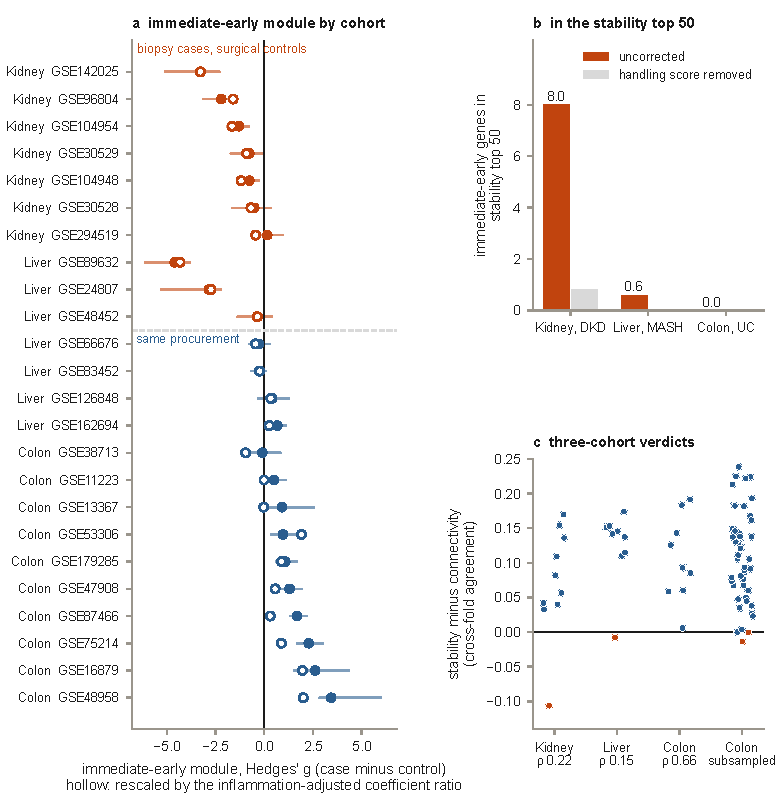
\includegraphics[width=\textwidth]{FigS5}
\caption{\textbf{Outside kidney, the immediate-early module follows procurement where it is
asymmetric and inflammation where it is not, and reaches the most reproducible genes mainly in
kidney.} \textbf{a}
Hedges' $g$ of the handling score, case minus control, with 95\% bootstrap intervals, for every
cohort whose procurement could be coded. Above the dashed line, biopsy cases against surgical or
donor controls; below, both arms obtained by the same procedure. Hollow points are not a second $g$: they are that $g$
multiplied by the ratio of the adjusted to the unadjusted standardised case coefficient from the
inflammation regression, which carries the adjustment onto the same axis. The two coefficients on
their own scale are in Supplementary File~7. \textbf{b} Mean number of immediate-early genes in the
stability-selection top 50 over leave-one-dataset-out folds on each tissue's five core cohorts,
uncorrected and after residualising on the handling score. \textbf{c} Stability selection minus
the connectivity comparator in cross-fold agreement for every three-cohort subset; orange points
are subsets in which the verdict reversed. Custom co-expression hub comparator; not the reference WGCNA implementation. $\rho$ is the median pairwise Spearman correlation of
gene-wise effect sizes across the five core cohorts. The rightmost column repeats colon with each
cohort subsampled to kidney case and control counts (five replicates of ten subsets). Filled
points in \textbf{a}, panel \textbf{b} and the first three columns of \textbf{c} test the
registered predictions; the inflammation adjustment, concordance and subsampling are post
hoc.}\label{fig:xtissue-full}
\end{figure}
\bibliographystyle{bib-vancouver}
\bibliography{dkd-references}
\end{document}
